


\begin{figure}[H]
    \centering
    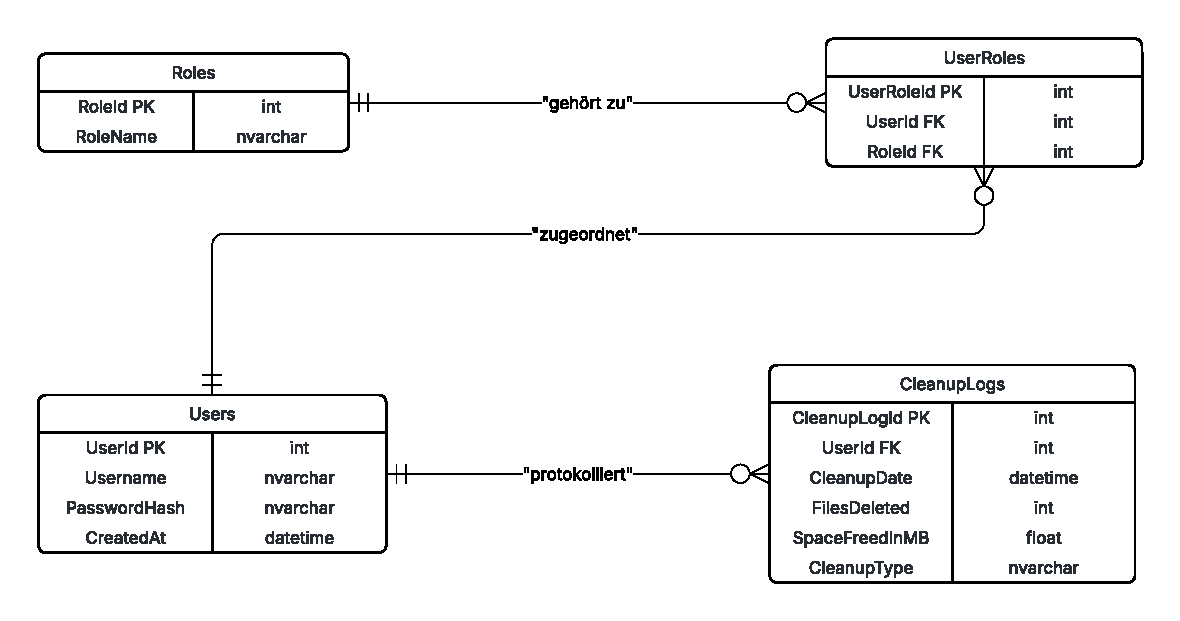
\includegraphics[width=\textwidth]{src/er_diagramm.pdf}
    \caption{ER-Diagramm der GarbageCollector-Datenbank}
\end{figure}


\setlength{\parskip}{0pt}
\setlength{\itemsep}{2pt}

\subsubsection*{Users (Benutzer)}
{\small
\begin{itemize}
    \item \textbf{UserId (PK)}: Eindeutige Kennung für jeden Benutzer.
    \item \textbf{Username}: Benutzername.
    \item \textbf{PasswordHash}: Gehashter Wert des Benutzerpassworts.
    \item \textbf{CreatedAt}: Zeitstempel bei Erstellung des Benutzers.
\end{itemize}
\textbf{Beziehungen:}
\begin{itemize}
    \item \textit{1:n} zu \textbf{CleanupLogs}: Ein Benutzer kann mehrere Bereinigungen durchgeführt haben.
    \item \textit{n:m} zu \textbf{Roles} über \textbf{UserRoles}.
\end{itemize}
}

\subsubsection*{Roles (Rollen)}
{\small
\begin{itemize}
    \item \textbf{RoleId (PK)}: Eindeutige Kennung der Rolle.
    \item \textbf{RoleName (UNQ)}: Rollenbezeichnung, z.\,B. „Admin“ oder „User“.
\end{itemize}
\textbf{Beziehung:}
\begin{itemize}
    \item \textit{1:n} zu \textbf{UserRoles}.
\end{itemize}
}

\subsubsection*{UserRoles (Benutzer-Rollen-Verknüpfung)}
{\small
\begin{itemize}
    \item \textbf{UserRoleId (PK)}: Eindeutige Kennung für jeden Eintrag.
    \item \textbf{UserId (FK)}: Verweis auf einen Benutzer.
    \item \textbf{RoleId (FK)}: Verweis auf eine Rolle.
\end{itemize}
\textbf{Beziehungen:}
\begin{itemize}
    \item \textit{n:1} zu \textbf{Users}, \textit{n:1} zu \textbf{Roles}.
\end{itemize}
}

\subsubsection*{CleanupLogs (Bereinigungsprotokolle)}
{\small
\begin{itemize}
    \item \textbf{CleanupLogId (PK)}: Eindeutige ID für den Protokolleintrag.
    \item \textbf{UserId (FK)}: Verweis auf den Benutzer.
    \item \textbf{CleanupDate}: Datum/Uhrzeit des Vorgangs.
    \item \textbf{FilesDeleted}: Anzahl gelöschter Dateien.
    \item \textbf{SpaceFreedInMB}: Freigegebener Speicherplatz in MB.
    \item \textbf{CleanupType}: Typ des Vorgangs (Standard, Junk, Duplicates).
\end{itemize}
\textbf{Beziehung:}
\begin{itemize}
    \item \textit{n:1} zu \textbf{Users}.
\end{itemize}
}
